

\chapter{Appendix} \label{Chapter:Appendix}

\section{2D Pulse sequences for PH-TOCSY and PH-HMQC}

The pulse sequences used for the PH-TOCSY and the PH-HMQC spectra are shown below.

\begin{center}
  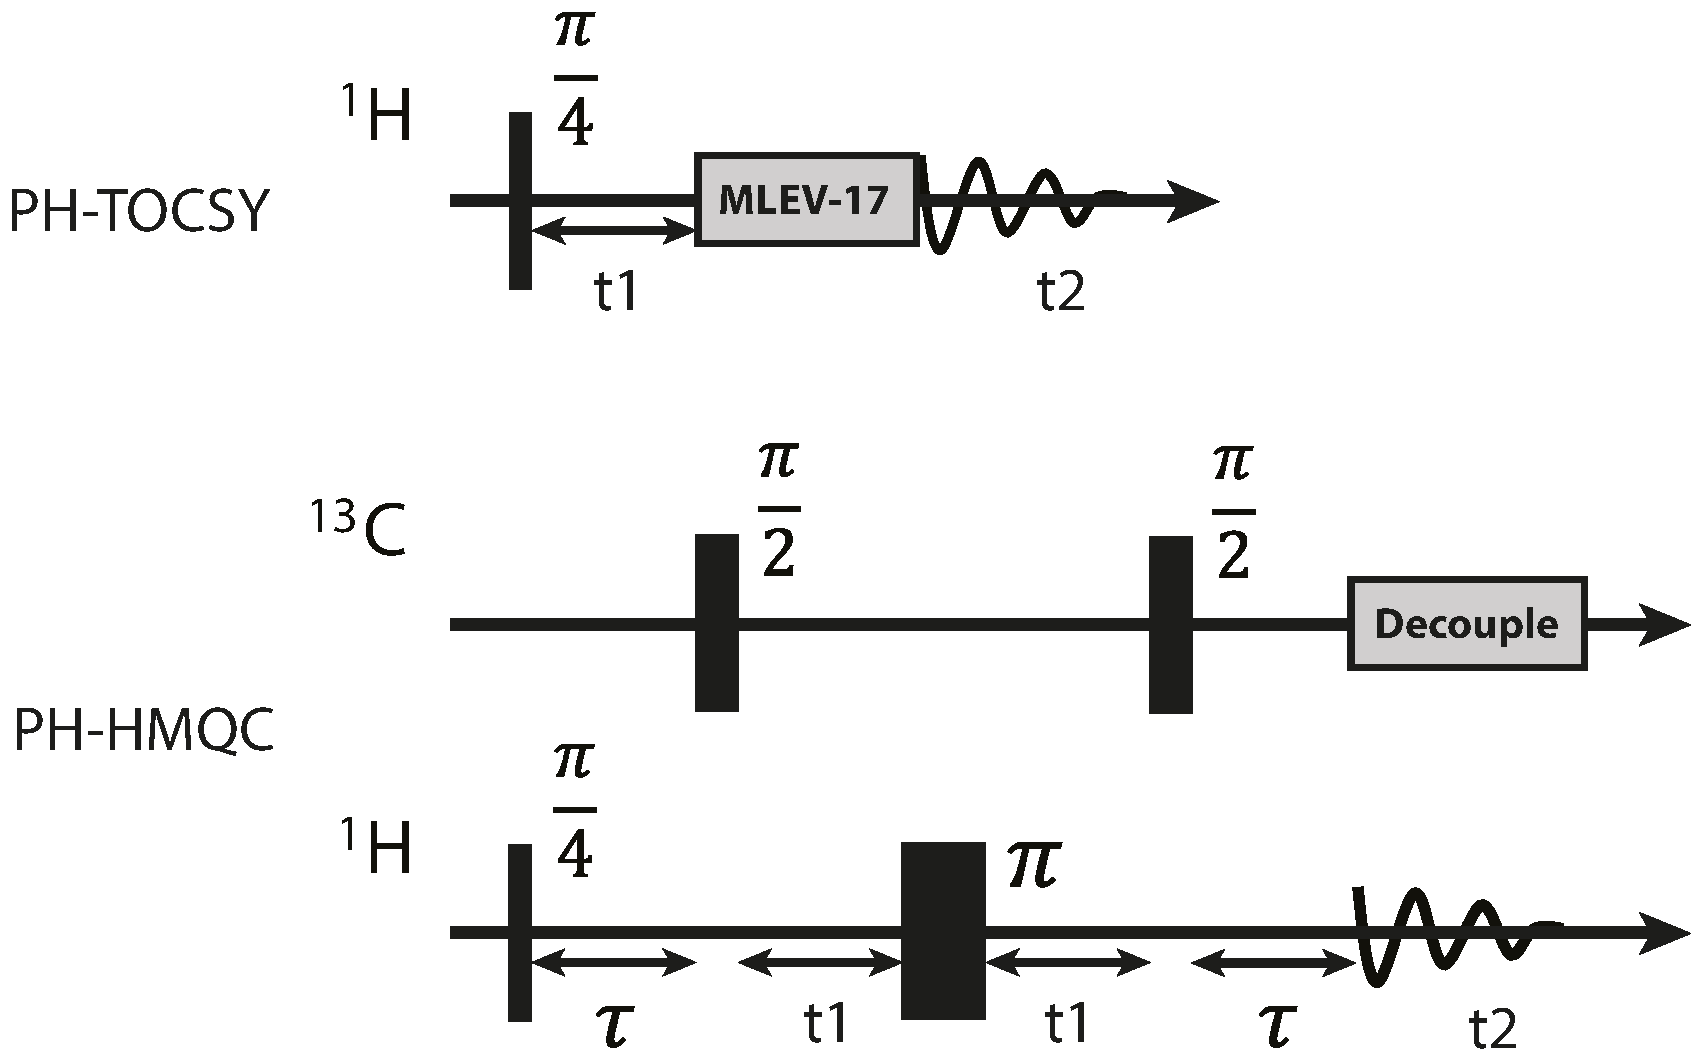
\includegraphics[width=7cm]{PH-TOCSY-HMQC-pulse-sequences.pdf}
\end{center}



\section{Arduino Firmware}

Below the firmware for the operation of the peristaltic pump is given.

\begin{lstlisting}

pump_driver_0.0.1

#define VALVE_A 3
#define VALVE_B 11
#define VALVE_C 2
#define VALVE_D 4
#define VALVE_E 5
#define VALVE_F 6
#define N_VALVES 6

int ValvePins[] = {VALVE_A, VALVE_B, VALVE_C, VALVE_D, VALVE_E,VALVE_F};

int AdvancePump[] = {VALVE_A, VALVE_B, VALVE_C};
int AdvanceValves[] = {LOW, LOW, LOW, HIGH, LOW, LOW};

int MixPump[] = {VALVE_F, VALVE_D, VALVE_B};
int MixValves[] = {HIGH, LOW, LOW, LOW, HIGH, LOW};


long bedTime = 0;


enum state  {QUIET, MIX, ADVANCE};

String stateDesc[] = {"idling.", "mixing", "pumping"} ;

state currentState;
state lastState;

const int MaxParams = 5;
String command;
String params[MaxParams];
int nparam=0;

float  freq = -1.0;
float lambda = 3.0;

void setup() {

  for(int k=0;k<N_VALVES;k++)
    {
      pinMode(ValvePins[k], OUTPUT);
      digitalWrite(ValvePins[k], LOW);
    }

   Serial.begin(115200);
   while(!Serial);
   Serial.println("Hello.");
}

void loop() {
  if( checkForCmd() ) processCmd()  ;
  if( millis() > bedTime ) gotoState(QUIET);

  switch (currentState) {
    case MIX :
      startPump(MixPump,3,freq,lambda) ;
      break ;

    case ADVANCE :
      startPump(AdvancePump,3,freq,lambda) ;
      break;

    default:
      break;
  }

  delay(10);
}


void gotoState(state newState)
{
  if(currentState != newState) {
    lastState = currentState;
    currentState = newState;

    Serial.print(stateDesc[newState]);

    switch(newState) {
      case MIX:
        for(int k=0;k<N_VALVES;k++) digitalWrite(ValvePins[k],MixValves[k]);
        Serial.print(" for ");
        Serial.print((bedTime-millis())/1000.0);
        Serial.println(" seconds.");
        break;

      case ADVANCE:
        for(int k=0;k<N_VALVES;k++) digitalWrite(ValvePins[k],AdvanceValves[k]);
        Serial.print(" for ");
        Serial.print((bedTime-millis())/1000.0);
        Serial.println(" seconds.");
        break;

      case QUIET:
        for(int k=0;k<N_VALVES;k++) digitalWrite(ValvePins[k],LOW);
        Serial.println();
        break;
    }


  }
}

bool checkForCmd()
{
   if(!Serial.available()) return(false);

   command = Serial.readStringUntil('\n');
   command.trim();
   int k;
   do {
      k=command.indexOf(' ');
      params[nparam++] = command.substring(0,k);
      command=command.substring(k);
      command.trim();
   } while(k>0 && nparam < MaxParams) ;

   /* Serial.println("command read."); */

   return(true);
}

void processCmd()
{

  command="";

  /* for(int k=0;k<nparam;k++) {
    Serial.println(params[k]);
  } */

  if(nparam>0) {

     if(params[0]=="mix") {
      bedTime = millis() + params[1].toFloat()*1000;
      gotoState(MIX);
    }

     else if (params[0]=="adv") {
      bedTime = millis() + params[1].toFloat()*1000;
      gotoState(ADVANCE);
     }

     else if(params[0]=="stop") {
      gotoState(QUIET);
      bedTime = millis();
     }

  }

  nparam=0;
}


void startPump(int *valves, int npins, float freq, float lambda)
{
  float psi;
  for(int k=0;k<npins;k++) {
    psi=cos( 2*PI*(k/lambda-freq*millis()/1000.)) ;
    if(psi>0)
        digitalWrite(valves[k],HIGH) ;
    else
      digitalWrite(valves[k],LOW);
  }
}

void stopPump(int *valves, int npins)
{
  for(int k=0;k<npins;k++)
    digitalWrite(valves[k],LOW);
}
\end{lstlisting}
